  \documentclass[12pt]{exam}
\usepackage{amsthm}
\usepackage{libertine}
\usepackage[utf8]{inputenc}
\usepackage[margin=1in]{geometry}
\usepackage{amsmath,amssymb}
\usepackage{multicol}
\usepackage[shortlabels]{enumitem}
\usepackage{siunitx}
\usepackage[spanish]{babel}
\usepackage{cancel}
\usepackage{graphicx}
\usepackage{float}
\usepackage{pgfplots}
\usepackage{listings}
\usepackage{tikz}


\pgfplotsset{width=10cm,compat=1.9}
\usepgfplotslibrary{external}
\tikzexternalize

\newcommand{\class}{Diseño y Análisis de Algoritmos} % This is the name of the course 
\newcommand{\examnum}{Documentación Proyecto 1} % This is the name of the assignment
\newcommand{\examdate}{\today} % This is the due date
\newcommand{\timelimit}{}





\begin{document}
\pagestyle{plain}
\thispagestyle{empty}

\noindent
\begin{tabular*}{\textwidth}{l @{\extracolsep{\fill}} r @{\extracolsep{6pt}} l}
	\textbf{\class} & \textbf{Name:} & \textit{Sergio Montoya}\\ %Your name here instead, obviously 
	\textbf{\examnum} &&\\
	\textbf{\examdate} &&
\end{tabular*}\\
\rule[2ex]{\textwidth}{2pt}
% ---

\section{Explicación Algoritmo}

\subsection{¿Que Hace?}

En esencia, lo que hace este algoritmo es dividir el problema en 3 trayectos (el de Indiana, el de Marion y el de Sallah) y los hace de manera lineal dejando en 0 el camino luego de recorrerlo. Ahora bien, para determinar cual es el mejor camino en cada uno de estos recorridos uso DP Bottom Up. En particular, lo que se hace es por cada recorrido se crea una matriz de la mitad del tamaño de la matriz original (Puesto que tenemos que llegar hasta la mitad de la matriz) y luego se recorre fila a fila. Por medio de una función que determina si esa celda entra 0 no se mira el máximo entre todas las posibles maneras en las que llegar y se suma el máximo de los posibles caminos con el valor de esta celda. Esto nos asegura que al llegar al final, en la ultima fila se encuentran los valores máximos que puede tener un camino que termine en esa celda y dado que siempre tenemos que llegar a esa fila entonces sabemos que el máximo es este camino. Luego de escoger nuestro máximo recorremos en reversa este camino y vamos convirtiendo en 0 todas las celdas que pasen por ahí. 

Ademas de esto, dado que las maldiciones son -1 esta garantizado que el mejor camino no pase por ahi. Ahora bien, para considerar el caso de que una casilla no pueda ser accedida pues esta yuxtapuesta por arriba solo con maldiciones entonces esta también se considera una maldición. De esta manera nos quitamos de encima la posibilidad de contar una celda que es imposible de acceder.

\subsection{¿Por que funciona?}

En este caso podemos explicar por que funciona en dos aspectos. Primero, por que el hecho de que lo hagamos linealmente no debería afectar y luego por que esto encuentra la mejor ruta.

\subsubsection{¿Por que se puede hacer lineal?}

En esencia el valor de una celda es el mismo si se lo lleva Indiana, Marion o Sallah. Por lo tanto, es equivalente hacer esto de manera lineal o hacerlo al tiempo. Siempre y cuando una vez uno de estos tres halla pasado por este camino lo retiremos de la matriz el resultado no debería cambiar.

\subsubsection{¿Por que Cada Camino es el mejor?}

El algoritmo implementado es esencialmente un algoritmo de DP clasico para encontrar el mejor camino en una matriz. Sin embargo, este tiene sumado que revisamos que se pueda llegar a esa casilla pues dado que tenemos un lugar de donde iniciar estas posibles casillas están bien definidas para nuestro caso. Por ejemplo la funcion $x \ge y$ es la manera en la que podemos determinar si una celda puede o no ser visitada por indiana Jones (Donde $x$ es la fila en la que esta y $y$ es la columna).

\subsection{Información de la Recurrencia}

Ahora bien, dado que utilizamos DP Bottom-Up es valioso que hablemos de la recurrencia utilizada. En este caso tenemos que para la función:

\begin{align*}
  mR\left( x, y \right) &= \begin{cases}
    0 & x == 0\\
    0 & !isAccessible(x)\\
    max_{-1 \le i \le 1}\left( mR\left( x - 1, y - i \right)  \right) + matrix(x, y) & \text{else}
  \end{cases} \\
.\end{align*}

Donde:
\begin{enumerate}
  \item \textbf{mR} es la función que devuelve la mayor recompensa posible para la celda $(x, y)$
  \item  $x$ es el numero de la fila en la que se encuentra
  \item $y$ es el numero de columna en la que se encuentra
  \item \textbf{isAccessible} es una función que determina si una celda puede ser accesible o no. Toma en consideración cosas como el camino máximo que puede recorrer el personaje, si es una maldición o si no se puede acceder a ella pues en algún punto del camino se bloquea por completo por maldiciones.
\end{enumerate}

Ahora bien, como se puede ver esto nos daría un diagrama de necesidades de la siguiente manera:
\begin{figure}[H]
  \centering
  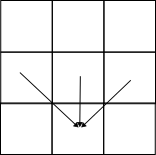
\includegraphics[width=0.4\textwidth]{IMG/img1.png}
  \caption{Diagrama de necesidades para determinar la mejor recompensa para una celda}
  \label{fig:IMG-img1-png}
\end{figure}

\section{Análisis de Complejidad}
\subsection{Temporal}

En este caso y dadas las similitudes solo calcularemos la complejidad de la función $calculateUp$ que la puede encontrar en el código a partir de la linea  $186$. Esto puesto que es la función mas importante y ademas la función inversa es equivalente pero se dividieron en dos para simplificarse. Si va al código encontrara ademas una pseudo tabla $CostVsTimes$. Ahora bien, es importante recalcar que en estos comentarios:
\begin{enumerate}
  \item $a$ es el numero de celdas accesibles para cada personaje.
  \item $n$ el numero de filas de la matriz original
  \item  $m$ el numero de columnas de la matriz original.
\end{enumerate}

Con esto en mente entonces la complejidad es:
\begin{align*}
  T(n, m) &= C_1 + O(n) + \frac{C_2}{2}n + \frac{C_3 + C_4 + C_{16}}{2} n\cdot m \\
	  &+ \left( O\left( 1 \right) + C_5 + C_6 + 3\left( C_7 + C_8 + C_9 + C_{10} + C_{11} + C_{12} + C_{13} + C_{14} + C_{15} - C_{16} \right)\right) a\\
	  T\left( n, m \right) &= O\left( n\cdot m \right) 
.\end{align*}
\subsection{Espacial}
En términos de complejidad Espacial en este caso se crea por cada recorrido una matriz de $\frac{n}{2}*m$ por lo tanto la complejidad de todo el algoritmo es:
\begin{align*}
  E\left( n, m \right) &= 3\frac{n}{2}*m\\
  E\left( n, m \right) &= O\left( n \cdot m \right)
.\end{align*}

\section{Preguntas}
\subsection{Primera Pregunta}

En este caso, dado que no se convierte en piedra esto seria el equivalente en la matriz de valores de DP a una celda que siempre vale 0. No tiene ningún castigo para las celdas yuxtapuestas pues se pueden atravesar sin ningún castigo pero no importa con cuanto valor se llegue ahí estas siempre valdrán 0. Es decir, se tendría que cambiar la función $isAccessible$ para que no tome en consideración las celdas que están bloqueadas por maldiciones.

\subsection{Segunda Pregunta}

En este caso, se encuentran las funciones que pueden determinar que celdas se pueden acceder iniciando desde cada celda (En general esto tiene la forma $abs\left( y - n \right) \le x$ para cuando se baja y $abs\left( y - n \right) \le abs(x - l)$ para cuando se sube. Con esto entonces podemos simplemente recorrer para cada uno de estos retirando en cada caso los tesoros del camino y ejecutando hasta que se acaben las personas o la matriz este vacía.



\end{document}
